\documentclass[a4paper, 11pt, english, greek]{article}

\usepackage{babel}
\usepackage{ucs}
\usepackage[utf8x]{inputenc}

\usepackage[T1]{fontenc}
%%\usepackage{lmodern}
\renewcommand{\ttdefault}{pcr}

\usepackage{subfig}
\usepackage[pdftex]{graphicx}
%%\usepackage{cite}
\usepackage{latexsym}

\title{Ρομποτική ΙΙ: Ευφυή Ρομποτικά Συστήματα \\ \vspace{12pt}
Εργασία 1: Κινηματικός έλεγχος ρομπότ με πλεονάζοντες βαθμούς ελευθερίας}
\author{Άλκης Γκότοβος}

\usepackage{hyperref}
\usepackage[all]{hypcap}

\begin{document}

\begin{titlepage}
	\maketitle
	\thispagestyle{empty}
\end{titlepage}

\section{Στόχος}
Στόχος της άσκησης είναι η δημιουργία περιβάλλοντος προσομοίωσης ενός ρομποτικού βραχίονα με 4 βαθμούς ελευθερίας.

Ο βραχίονας θα εκτελεί μία \emph{πρωτεύουσα εργασία}, η οποία συνίσταται στην παραμονή του τελικού στοιχείου
δράσης πάνω σε μία κατακόρυφη ευθεία.
Παράλληλα θα εκτελείται και μία \emph{δευτερεύουσα εργασία}, η οποία συνίσταται στην αποφυγή δύο κυκλικών εμποδίων,
τα οποία θα μπορούν να κινηθούν από το χρήστη με το πάτημα δύο κουμπιών.

\section{Γενικό σχήμα ελέγχου}
Για την προσομοίωση της κίνησης του ρομποτικού βραχίονα, θα χρησιμοποιηθεί το \emph{σχήμα ελέγχου τροχιάς επιλυμένης
ταχύτητας}.

Το γεωμετρικό μοντέλο του βραχίωνα με 4 παράλληλες στροφικές αρθρώσεις είναι απλό και δε θα αναφερθεί εδώ.

Το κομβικό σημείο στο έλεγχο επιλυμένης ταχύτητας είναι η λύση του αντιστρόφου κινηματικού προβλήματος, δηλαδή
η εύρεση των απαιτούμενων ταχυτήτων των αρθρώσεων, δεδομένης της επιθυμητής ταχύτητας του τελικού στοιχείου δράσης.
Στις επόμενες δύο ενότητες θα δείξουμε πώς επιλύουμε το πρόβλημα αυτό, ώστε να πετύχουμε την εκτέλεση των δύο
επιθυμητών εργασιών.

\section{Πρωτεύουσα εργασία}
Για την εκτέλεση της πρωτεύουσας εργασίας απαιτείται το τελικό στοιχείο δράσης να παραμένει επί μιας κατακόρυφης
ευθείας, ενώ ο προσανατολισμός δεν παίζει ρόλο.

Αυτό σημαίνει ότι αρκεί ένας βαθμός ελευθερίας για την εργασία αυτή.
Επιπλέον, επειδή η ευθεία είναι κατακόρυφη, ο κινηματικός περιορισμός του τελικού στοιχείου δράσης τίθεται μόνο
για τη συνιστώσα \textlatin{x}.
Συνεπώς, ο Ιακωβιανός πίνακας της πρωτεύουσας εργασίας θα αφορά μόνο την προαναφερθείσα συνιστώσα, δηλαδή θα είναι
ο πίνακας-γραμμή

\begin{center}
	$\mathbf{J_{1}} = [\frac{\displaystyle \partial p_{x}}{\displaystyle \partial q_{1}},
	                   \frac{\displaystyle \partial p_{x}}{\displaystyle \partial q_{2}},
	                   \frac{\displaystyle \partial p_{x}}{\displaystyle \partial q_{3}},
	                   \frac{\displaystyle \partial p_{x}}{\displaystyle \partial q_{4}}]$
\end{center}
Τότε, η λύση του αντιστρόφου κινηματικού προβλήματος, που ικανοποιεί τον περιορισμό της πρωτεύουσας εργασίας,
έχει τη μορφή

\begin{center}
	$\mathbf{\dot{q}} = \mathbf{J_{1}^{+}} \mathbf{\dot{p}} +
	         (\mathbf{I} - \mathbf{J_{1}^{+}} \mathbf{J_{1}}) \mathbf{k_{0}}$
\end{center}
Ο πίνακας $\mathbf{J_{1}^{+}}$ είναι ο ψευδοαντίστροφος του $\mathbf{J_{1}}$.
To $\mathbf{k_{0}}$ μπορεί να είναι οποιοδήποτε διάνυσμα, αφού ο δεύτερος όρος του παραπάνω αθροίσματος θα ανήκει
σε κάθε περίπτωση στο μηδενικό χώρο της πρωτεύουσας εργασίας.

\section{Δευτερεύουσα εργασία}
Για να εκτελείται η δευτερεύουσα εργασία, δηλ. να αποφεύγονται τα εμπόδια, θα πρέπει να προσδιορίσουμε κατάλληλο διάνυσμα
$\mathbf{k_{0}}$ στη λύση της προηγούμενης ενότητας.
Το $\mathbf{k_{0}}$ προφανώς θα εξαρτάται από τη διάταξη του βραχίονα, αλλά και από τις θέσεις των εμποδίων.

Ένας τρόπος ικανοποίησης της δευτερεύουσας εργασίας είναι μέσω μιας συνάρτησης δυναμικού $\mathbf{h}$, η οποία θα έχει
ελάχιστα στις επιθυμητές διατάξεις, ενώ οι τιμές της θα αυξάνονται όσο ο βραχίονας πλησιάζει τα εμπόδια.

Τότε ο στόχος θα είναι η \emph{ελαχιστοποίηση} της $\mathbf{h}$ και κατά συνέπεια μπορούμε να θέσουμε το $\mathbf{k_{0}}$
ίσο με την κλίση της $\mathbf{h}$, οπότε η λύση της προηγούμενης ενότητας μπορεί πλέον να εκφραστεί ως

\begin{center}
	$\mathbf{\dot{q}} = \mathbf{J_{1}^{+}} \mathbf{\dot{p}} -
	         k_{h} (\mathbf{I} - \mathbf{J_{1}^{+}} \mathbf{J_{1}}) \nabla\mathbf{h}$
\end{center}
Εφαρμόζουμε ουσιαστικά τη μέθοδο του \textlatin{gradient descent} στον μηδενικό χώρο της πρώτης υποεργασίας.
Ο συντελεστής $k_{h}$ είναι η σταθερά κέρδους της μεθόδου αυτής και δείχνει πόσο μεγάλα βήματα κάνουμε στην κατεύθυνση
του \textlatin{gradient} σε κάθε χρονική στιγμή.

Η επιλογή της συνάρτησης δυναμικού $\mathbf{h}$ δεν είναι απλή υπόθεση.
Η αρχική ιδέα ήταν να χρησιμοποιηθεί μία συνάρτηση ηλεκτροστατικού δυναμικού, θεωρώντας τα δύο εμπόδια
ως θετικά φορτισμένες σημειακές πηγές και κάποια σημεία του βραχίωνα (π.χ. κάποιες αρθρώσεις) ως επίσης
θετικά φορτισμένες σημειακές πηγές, έτσι ώστε τα εμπόδια να απωθούν το βραχίωνα.

Μέσω πειραματισμού, φάνηκε ότι αρκεί να τοποθετηθούν κάποιες σημειακές πηγές στον τρίτο σύνδεσμο του βραχίωνα,
επειδή στο συγκεκριμένο πρόβλημα ο σύνδεσμος αυτός βρίσκεται μεταξύ των εμποδίων.

Επίσης, η συνάρτηση του απλού ηλεκτροστατικού δυναμικού (αντιστρόφως ανάλογο της απόστασης των πηγών)
δεν είναι αρκετά απότομη για το συγκεκριμένο πρόβλημα, με αποτέλεσμα να έχουμε μεγάλους χρόνους απόκρισης του
βραχίωνα, όταν μετατοπίζονται τα εμπόδια.

Για αυτό επιλέχθηκε μία αρκετά πιο απότομη συνάρτηση δυναμικού για κάθε ζεύγος σημειακών πηγών
με εξίσωση της μορφής (\textlatin{Fermi-Dirac})

\begin{center}
	$h(r) = \frac{\displaystyle a}{\displaystyle b + e^{c r}}$
\end{center}
Οι συντελεστές $a$, $b$ και $c$ επιλέχθηκαν πειραματικά, ώστε η διάταξη να έχει σχετικά γρήγορη απόκριση
στη μετακίνηση των εμποδίων και παράλληλα να μην παρουσιάζονται πολλές ταλαντώσεις και ασταθείς συμπεριφορές.
Το ίδιο ισχύει και για τον προσδιορισμό του συντελεστή $k_{h}$.

\section{Πειραματικά αποτελέσματα}
Στα σχήματα 1 έως 10 φαίνονται κάποια στιγμιότυπα του βραχίωνα για διάφορες θέσεις των εμποδίων.

Η συμπεριφορά του βραχίονα είναι αρκετά καλή σε γενικές γραμμές.
Μπορούμε να δούμε ότι η πρωτεύουσα εργασία εκτελείται πάντα επιτυχώς.
Η δευτερεύουσα εργασία εκτελείται αρκετά καλά και έχει σχετικά μικρούς χρόνους απόκρισης.

Κάποια προβλήματα παρουσιάζονται στις ιδιόμορφες διατάξεις (π.χ. αρχική διάταξη του βραχίονα), όπου
οι χρόνοι απόκρισης στη μετακίνηση των εμποδίων είναι αρκετά μεγαλύτεροι.
Αυτό είναι αναμενόμενο, αφού σε αυτές τις διατάξεις ο βραχίονας χάνει έναν ή περισσότερους βαθμούς
ελευθερίας, οπότε περιμένουμε η συμπεριφορά του να είναι χειρότερη.

Από την άλλη η αρκετά απότομη συνάρτηση δυναμικού που επιλέχθηκε για να μειώσει τους χρόνους απόκρισης
(κυρίως στις ιδιόμορφες διατάξεις που προαναφέρθηκαν),
οδηγεί ορισμένες φορές το σύστημα σε κάποιες μικρές ταλαντώσεις.

Τελικά, έγινε προσπάθεια να επιλεχθούν (πειραματικά) κατάλληλες παράμετροι, ώστε να βρεθεί μία μέση λύση
και τα δύο φαινόμενα που αναφέρθηκαν παραπάνω να παραμένουν σε αποδεκτά επίπεδα.

\begin{figure}[htb]
  \centering
  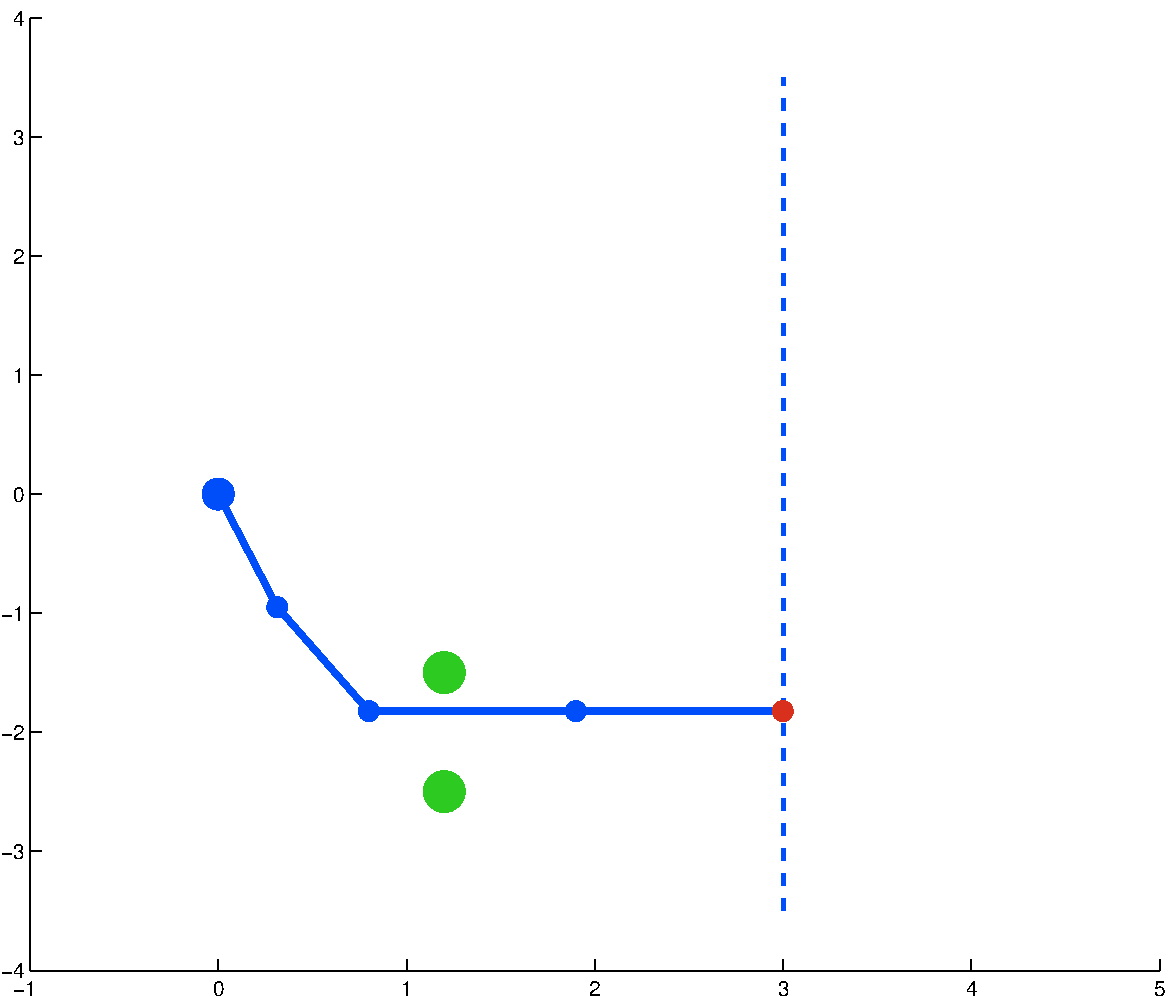
\includegraphics[width=300px]{test1}
  \caption{}
\end{figure}

\begin{figure}[htb]
  \centering
  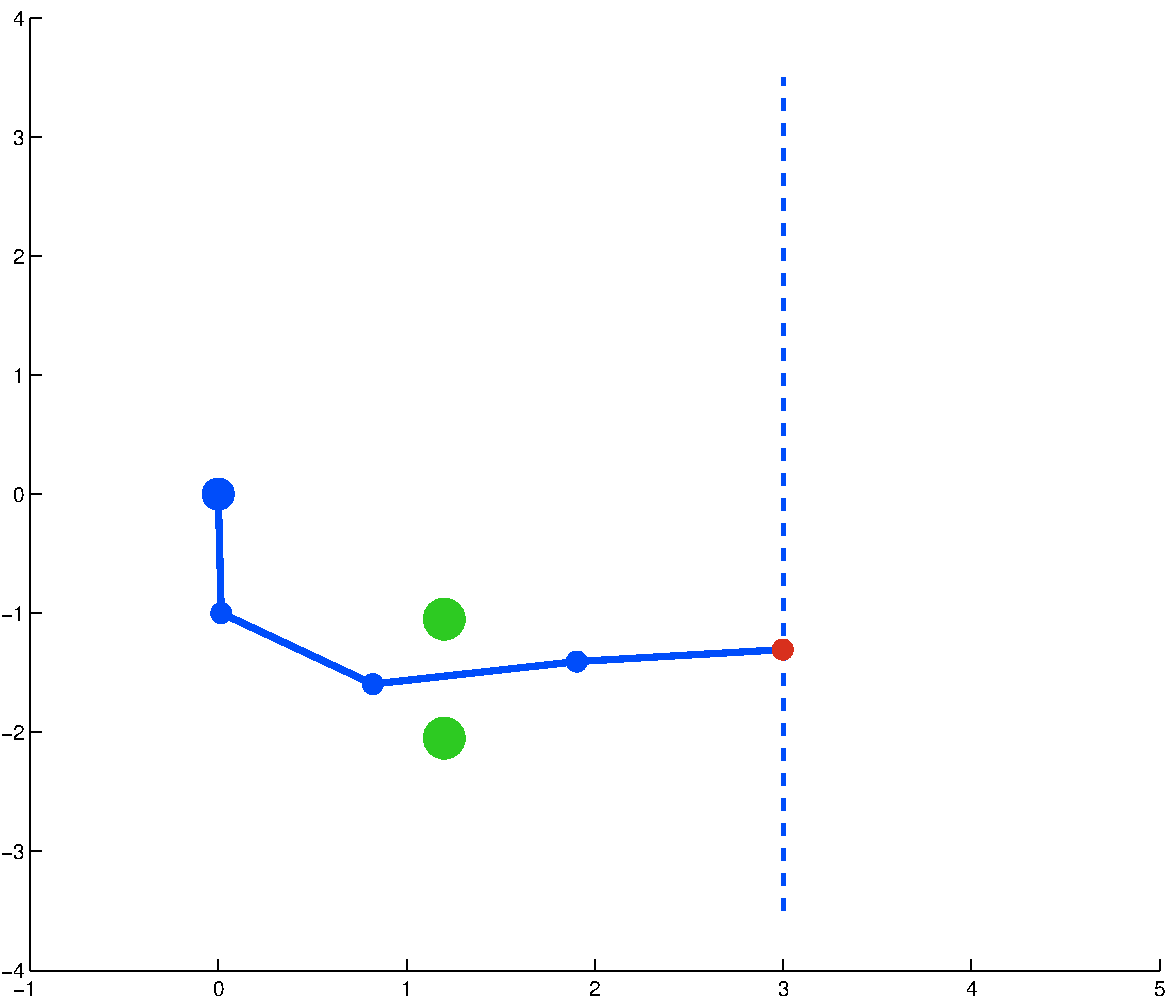
\includegraphics[width=300px]{test2}
  \caption{}
\end{figure}

\begin{figure}[htb]
  \centering
  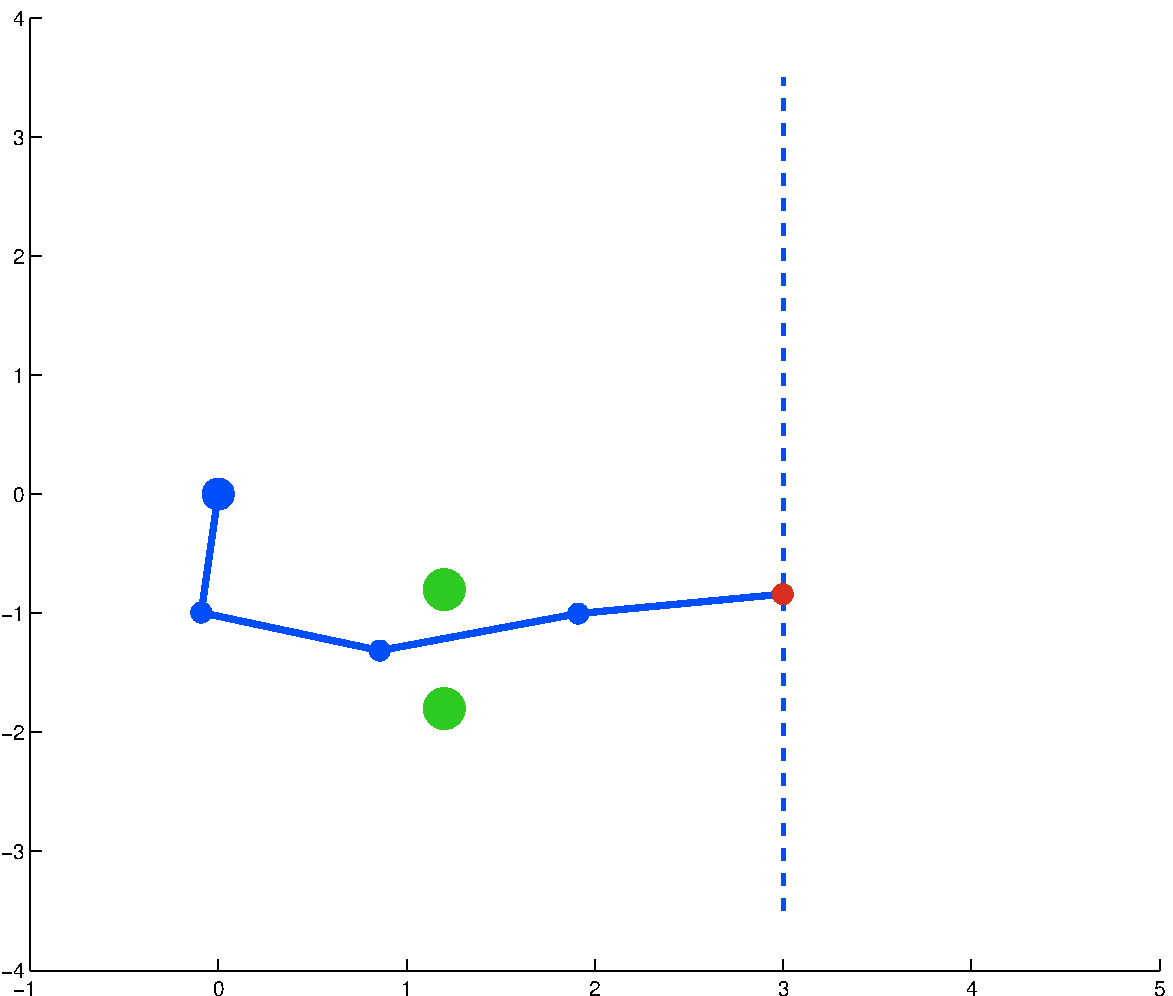
\includegraphics[width=300px]{test3}
  \caption{}
\end{figure}

\begin{figure}[htb]
  \centering
  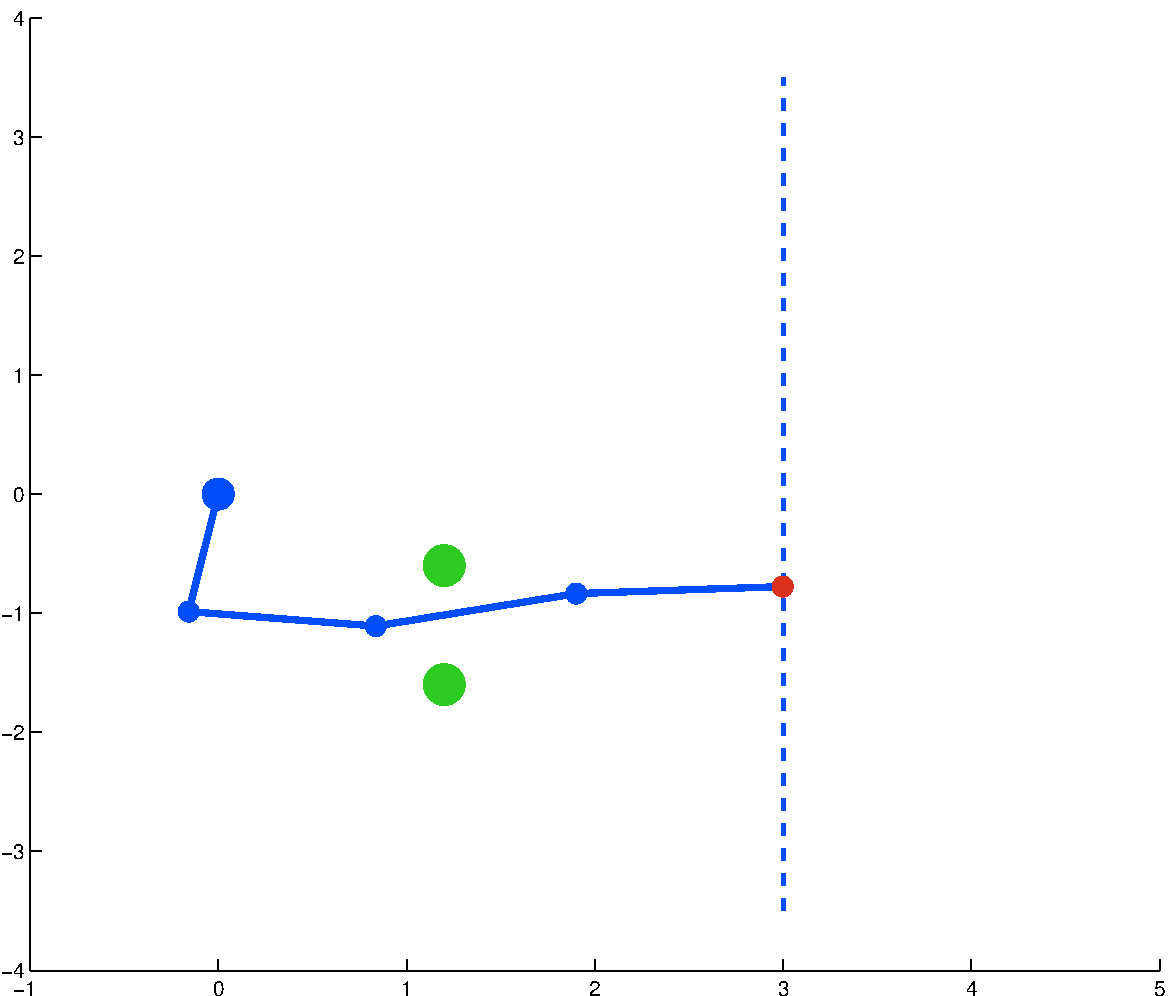
\includegraphics[width=300px]{test4}
  \caption{}
\end{figure}

\begin{figure}[htb]
  \centering
  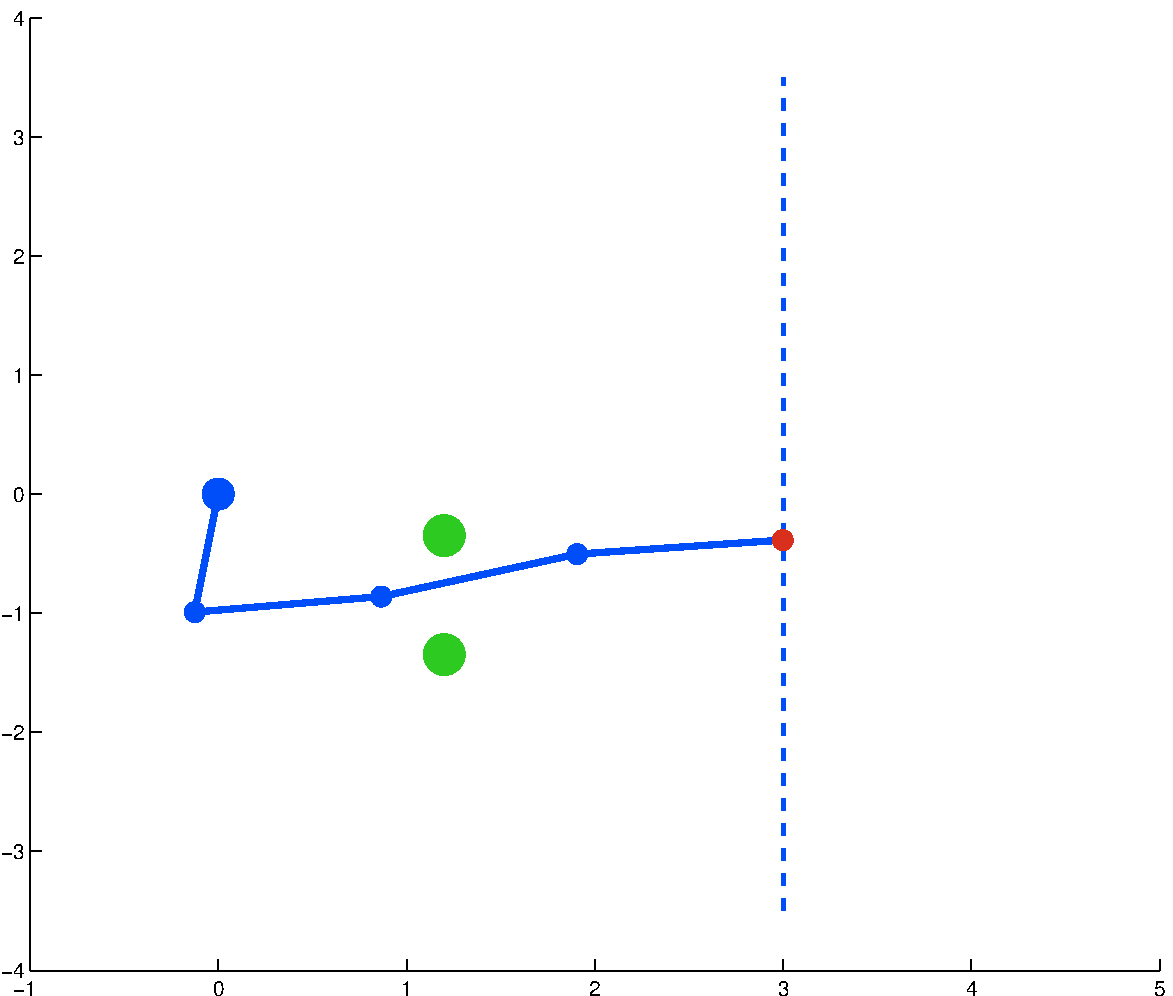
\includegraphics[width=300px]{test5}
  \caption{}
\end{figure}

\begin{figure}[htb]
  \centering
  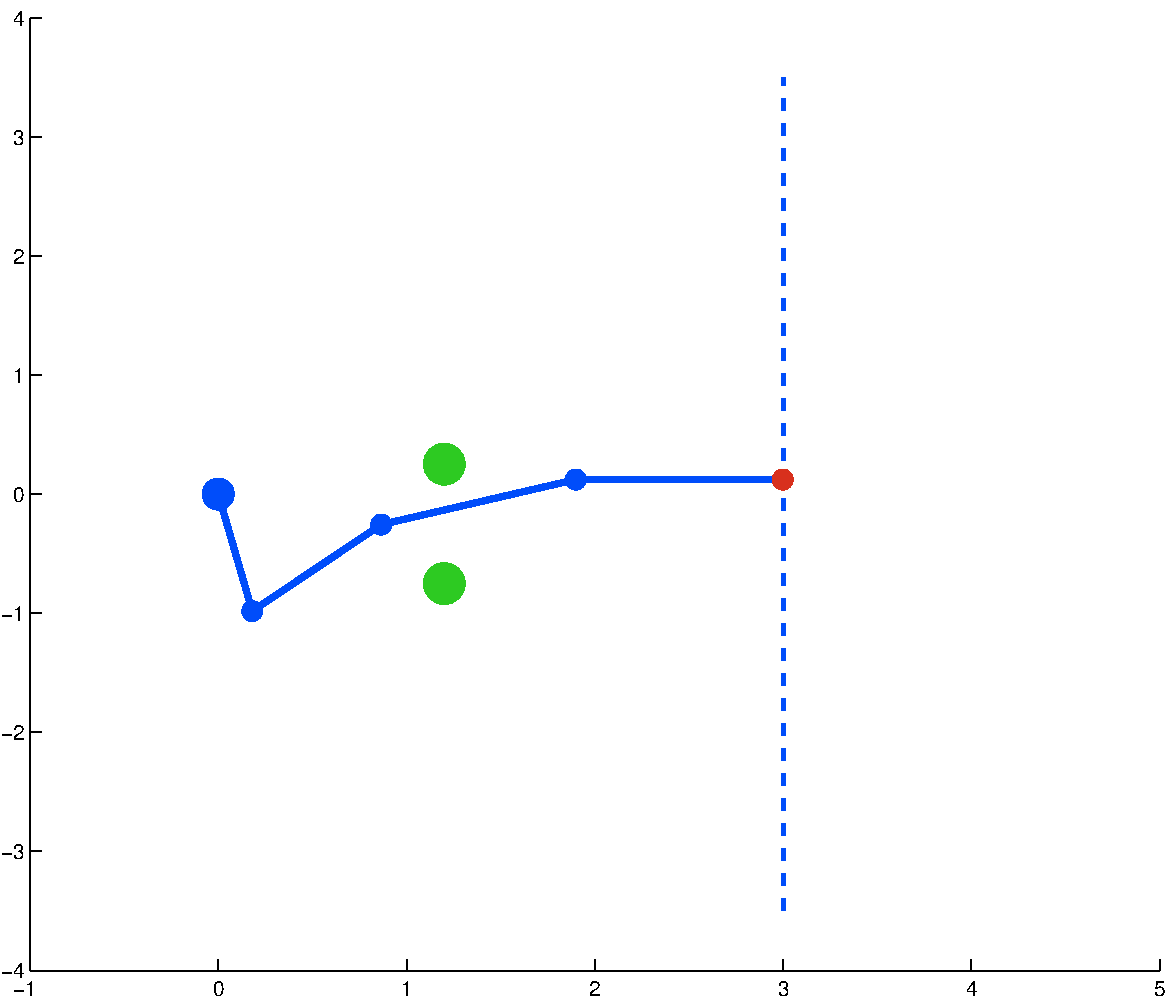
\includegraphics[width=300px]{test6}
  \caption{}
\end{figure}

\begin{figure}[htb]
  \centering
  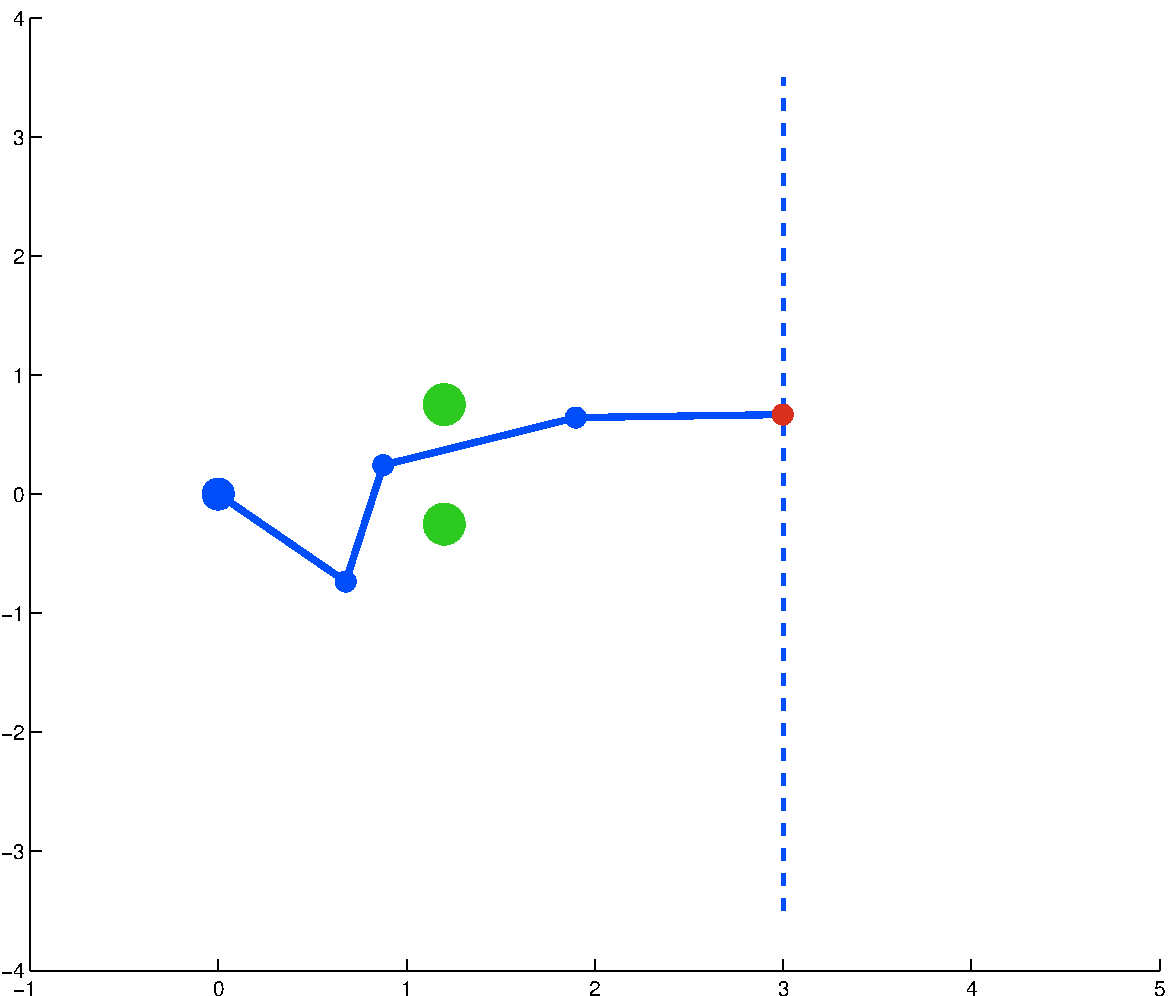
\includegraphics[width=300px]{test7}
  \caption{}
\end{figure}

\begin{figure}[htb]
  \centering
  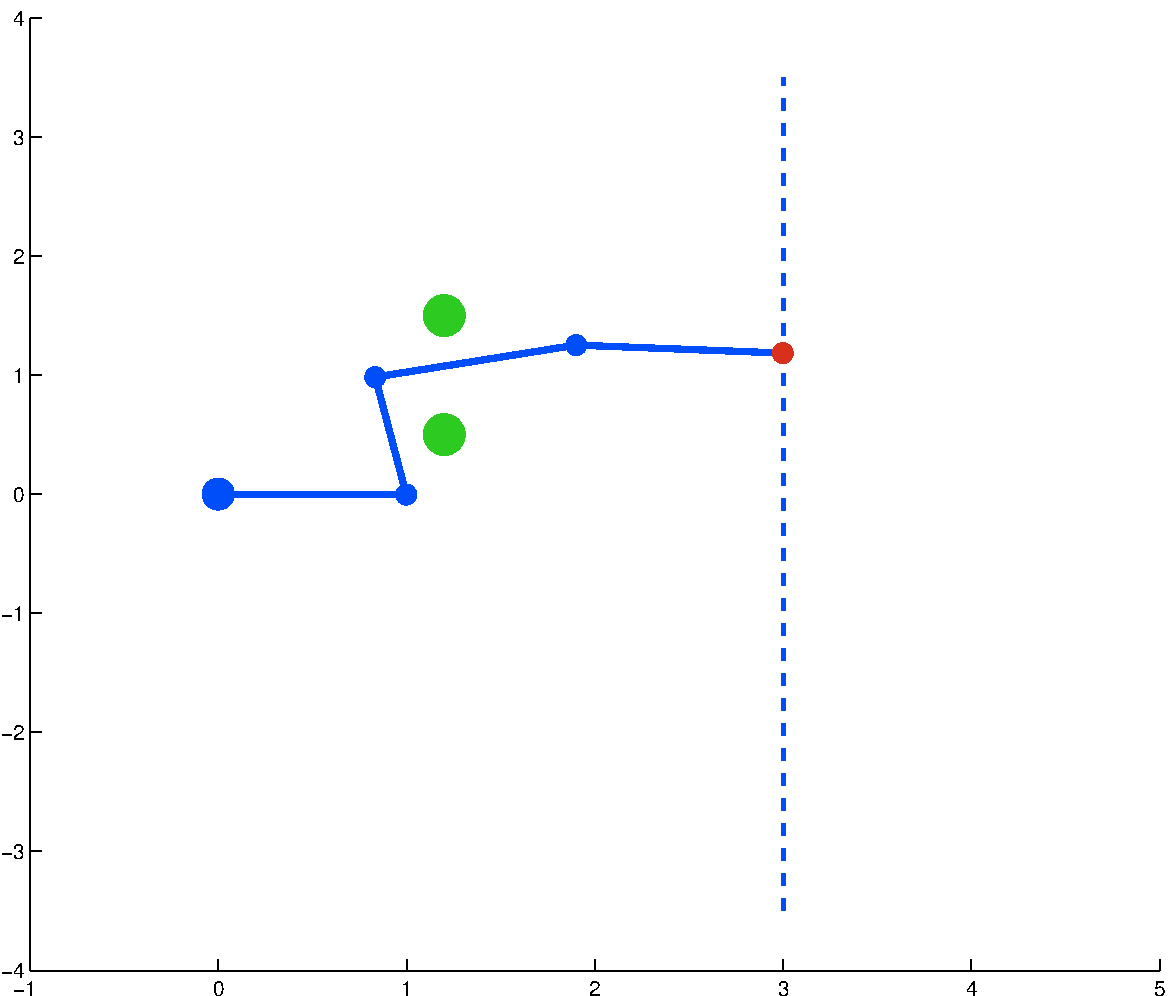
\includegraphics[width=300px]{test8}
  \caption{}
\end{figure}

\begin{figure}[htb]
  \centering
  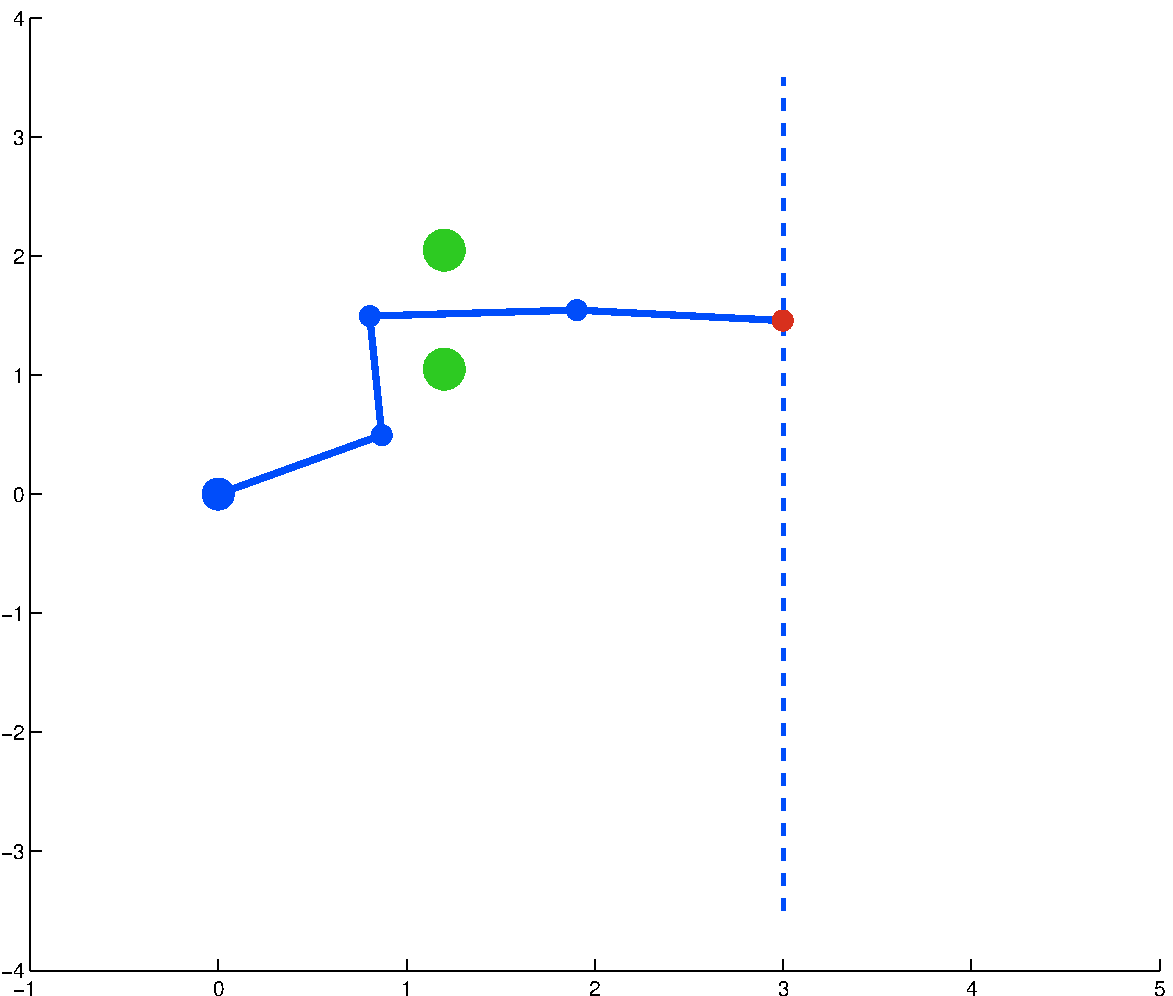
\includegraphics[width=300px]{test9}
  \caption{}
\end{figure}

\begin{figure}[htb]
  \centering
  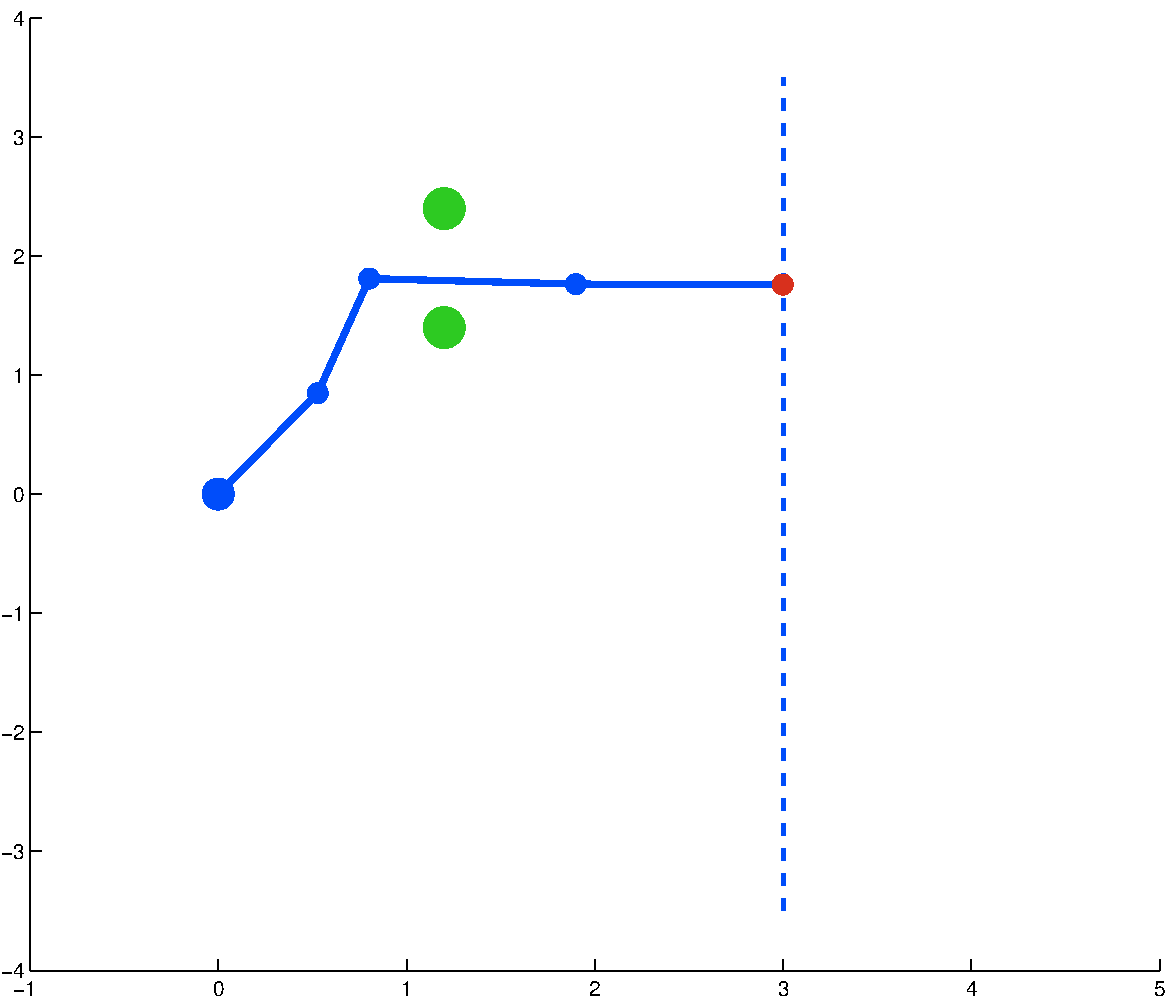
\includegraphics[width=300px]{test10}
  \caption{}
\end{figure}

\end{document}